\documentclass[10pt,letterpaper,twocolumn]{article}

\usepackage[top=2.1cm,left=2.0cm,right=2.0cm,footskip=2.0cm]{geometry}
\usepackage[utf8]{inputenc}     % for Unicode
\usepackage{cite}               % citation
\usepackage[dvipdfmx]{hyperref} % links
\usepackage{caption}            % caption
\usepackage{microtype}          % improves typesetting in LaTeX
\usepackage{graphicx}
\usepackage{color} % ex.) \textcolor{color}{text}

\begin{document}

\twocolumn[
    \begin{flushleft}
        {\Large
        \textbf\newline{An Extention of R-Tree for Periodic Boundary Conditions}
        }
        \newline
        \\
        Toru Niina \textsuperscript{1}
        \\
        \bigskip
        \bf{1.} Department of Biophysics, Graduate School of Science,
                Kyoto University, Kyoto 606-8502, Japan
        \\
        \bigskip
        * niina@theory.biophys.kyoto-u.ac.jp
    \end{flushleft}

    \section*{Abstract}
    Spatial searching is an important operation for physical, chemical, and
    biological simulations which run mostly on periodic boundary conditions.
    An R-Tree is a widely used data structure to manage spatial data objects and
    it is capable of processing a spatial searching query in an efficient way.
    Currently, several methods to handle an R-Tree on periodic boundary
    conditions have been proposed. Those methods keep the underlying R-Tree
    structure intact but modify queries or entire system. In this paper, I
    propose a new method to make the spatial structure of R-Tree itself along
    the periodic boundary conditions introducing a set of operations for
    rectangles on the condition. It will remove the requirements for extensional
    queries or copies of objects.
    \bigskip
]

\section*{Introduction} % the '*' after section prevents numbering
Computational simulations are the essential tools for scientific study, such as
investigating behaviors of large and complex biochemical models. To perform
such a huge scale simulation, both large amount of computational resources and
efficient simulation softwares are required.

    In most cases, spatial search for objects satisfying certain geometrical
conditions is one of the most costly processes. Generally, an efficient method
for spatial search drastically accelerates not only the whole simulation
processes, but also the data analysis of simulation results.

    An R-Tree is a widely used data structure representing bounding volume
hierarchies (BVH) by using axis-aligned bounding box (AABB) for all its entries
% [\ref{Gutmann-RTree-1984}].
As its efficiency, many of its variants have been proposed [\textcolor{red}{TODO}].
add reference for R*, Hilbelt-R, STR-R, PriorityR, ...

    In order to use it with periodic boundary conditions (PBC), currently,
two methods are proposed[\textcolor{red}{TODO}]. The method visually described in
figure \ref{fig1} A copies all the objects in the simulation system
along each periodic boundaries. Although it can search objects associated with
the adjacent periodic images in the same way as normal R-Tree, it consumes
memory $3^D$ fold a lot (here $D$ reprecents a number of dimension). Figure
\ref{fig1} B showes another method that contains only one image,
copying query AABB in the same manner as copying whole system.

    Here I propose the novel method to apply PBC to R-Tree. The main idea is
applying the PBC to each operations of AABBs that are performed in each steps to
maintain an R-Tree. With this method, it is not needed to copy objects or query
AABBs at all. Moreover, using the information about the boundary condition,
it is expected that the size of each AABBs associated with each nodes decreases
relative to the other methods in some cases, suggesting that the spatial search
become more efficient.

    In section 2, I will show the methods that can be used to
grow and maintain the R-Tree structure. In section 3, I will show the performance
results when it is used in the biochemical simulation. In seciton 4, I will make
a summary of this paper and introduce the library to use my method in C++.

\begin{figure}[hbt]
    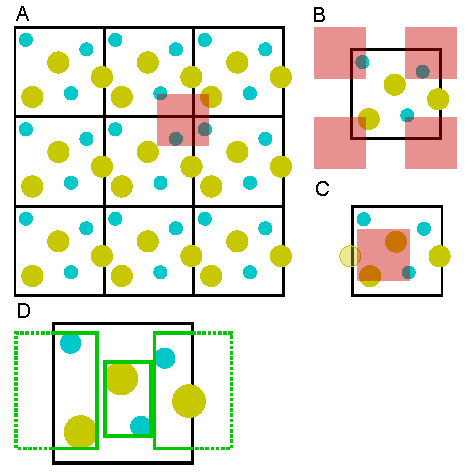
\includegraphics[width=6.5cm, bb=0 0 567 567]{fig1.eps}
    \caption{this is an example figure for the R-Tree structure}
    \label{fig1}
\end{figure}

\section*{Methods}

\paragraph{Paragraph.}
Lorem ipsum dolor sit amet, consectetur adipiscing elit. Aliquam bibendum
finibus diam, gravida sagittis lorem gravida vitae. Interdum et malesuada fames
ac ante ipsum primis in faucibus. Nulla in diam tristique ante posuere
tristique. Donec interdum purus sit amet nisl accumsan consectetur. Fusce
aliquet libero mi, quis ornare dolor congue ullamcorper. Nulla nulla urna,
molestie in urna sed, lacinia volutpat eros. Ut mi libero, elementum scelerisque
ipsum vel, hendrerit fermentum turpis. Aliquam sit amet leo sodales, egestas
augue id, fermentum nulla. Aenean vel cursus ante, et pellentesque eros. Nulla
ac neque nec justo posuere commodo sit amet sit amet justo. Aliquam tincidunt
tempor ex nec tincidunt. In ullamcorper vehicula lobortis.

\subsection*{Formulas.}
Lorem ipsum dolor sit amet, consectetur adipiscing elit. Aliquam bibendum
finibus diam, gravida sagittis lorem gravida vitae. Interdum et malesuada fames
ac ante ipsum primis in faucibus. Nulla in diam tristique ante posuere
tristique. Donec interdum purus sit amet nisl accumsan consectetur. Fusce
aliquet libero mi, quis ornare dolor congue ullamcorper. Nulla nulla urna,
molestie in urna sed, lacinia volutpat eros. Ut mi libero, elementum scelerisque
ipsum vel, hendrerit fermentum turpis. Aliquam sit amet leo sodales, egestas
augue id, fermentum nulla. Aenean vel cursus ante, et pellentesque eros. Nulla
ac neque nec justo posuere commodo sit amet sit amet justo. Aliquam tincidunt
tempor ex nec tincidunt. In ullamcorper vehicula lobortis.
% \begin{center}
\begin{eqnarray}
    f(x) &=& \mathrm{e}^x \nonumber\\
    g(x) &=& \log(x)      \nonumber
\end{eqnarray}
% \end{center}

\section*{Results}
\subsection*{subsection 1}
Lorem ipsum dolor sit amet, consectetur adipiscing elit. Aliquam bibendum
finibus diam, gravida sagittis lorem gravida vitae. Interdum et malesuada fames
ac ante ipsum primis in faucibus. Nulla in diam tristique ante posuere
tristique. Donec interdum purus sit amet nisl accumsan consectetur. Fusce
aliquet libero mi, quis ornare dolor congue ullamcorper. Nulla nulla urna,
molestie in urna sed, lacinia volutpat eros. Ut mi libero, elementum scelerisque
ipsum vel, hendrerit fermentum turpis. Aliquam sit amet leo sodales, egestas
augue id, fermentum nulla. Aenean vel cursus ante, et pellentesque eros. Nulla
ac neque nec justo posuere commodo sit amet sit amet justo. Aliquam tincidunt
tempor ex nec tincidunt. In ullamcorper vehicula lobortis.

\subsection*{subsection 2}
Lorem ipsum dolor sit amet, consectetur adipiscing elit. Aliquam bibendum
finibus diam, gravida sagittis lorem gravida vitae. Interdum et malesuada fames
ac ante ipsum primis in faucibus. Nulla in diam tristique ante posuere
tristique. Donec interdum purus sit amet nisl accumsan consectetur. Fusce
aliquet libero mi, quis ornare dolor congue ullamcorper. Nulla nulla urna,
molestie in urna sed, lacinia volutpat eros. Ut mi libero, elementum scelerisque
ipsum vel, hendrerit fermentum turpis. Aliquam sit amet leo sodales, egestas
augue id, fermentum nulla. Aenean vel cursus ante, et pellentesque eros. Nulla
ac neque nec justo posuere commodo sit amet sit amet justo. Aliquam tincidunt
tempor ex nec tincidunt. In ullamcorper vehicula lobortis.

\section*{Discussion}

Lorem ipsum dolor sit amet, consectetur adipiscing elit. Aliquam bibendum
finibus diam, gravida sagittis lorem gravida vitae. Interdum et malesuada fames
ac ante ipsum primis in faucibus. Nulla in diam tristique ante posuere
tristique. Donec interdum purus sit amet nisl accumsan consectetur. Fusce
aliquet libero mi, quis ornare dolor congue ullamcorper. Nulla nulla urna,
molestie in urna sed, lacinia volutpat eros. Ut mi libero, elementum scelerisque
ipsum vel, hendrerit fermentum turpis. Aliquam sit amet leo sodales, egestas
augue id, fermentum nulla. Aenean vel cursus ante, et pellentesque eros. Nulla
ac neque nec justo posuere commodo sit amet sit amet justo. Aliquam tincidunt
tempor ex nec tincidunt. In ullamcorper vehicula lobortis.

\bibliography{library}
\bibliographystyle{abbrv}

\end{document}
